% MapOSMatic - Libre Software Meeting 2012 presentation
% -*- coding: utf-8; mode: LaTeX -*-

% Copyright (C) 2010 Maxime Petazzoni <maxime.petazzoni@bulix.org>
%                    Thomas Petazzoni <thomas.petazzoni@enix.org>
% Distributed under the terms of the Creative Commons CC-by-sa 3.0

\documentclass{beamer}
\usepackage[utf8]{inputenc}
\usepackage[american]{babel}

\mode<presentation>
\usetheme{MapOSMatic}
\setbeamercovered{dynamic}

\title{MapOSMatic: free city maps for everyone!}
\author{Thomas {\sc Petazzoni}}
\date{July 10th, 2012}

\begin{document}

%%%%%%%%%%%%%%%%%%%%%%%%%%%%%%%%%%%%%%%%%%%%%%%%%%%%%%%%%%%%%%%%%%%%%%%

\begin{frame}
  \begin{center}
    \Huge
    MapOSMatic, free city maps for everyone!\\
    \vspace{2cm}
    \begin{columns}
      \column{0.6\textwidth}
      \normalsize
      Thomas Petazzoni\\
      \path{thomas.petazzoni@enix.org}\\
      Libre Software Meeting 2012\\
      \url{http://www.maposmatic.org}\\
      \column{0.4\textwidth}
      \includegraphics[height=0.3\textheight]{geneve-small.png}
    \end{columns}
  \end{center}
\end{frame}

\begin{frame}{Thomas Petazzoni}
  \begin{itemize}
  \item {\bf Embedded Linux engineer} and trainer at Free Electrons
  \item Regular contributor to the {\bf Buildroot} project, an open-source
    embedded Linux build system
  \item Contributor to the Linux {\bf kernel}
  \item Active in the free software community: founder of {\em
      Toulibre}, founder of the {\em Agenda du Libre}
  \item {\bf One of the developer of MapOSMatic}, together with
    David Decotigny, Gaël Utard, Maxime Petazzoni, David Mentré,
    Frédéric Lehobey, Étienne Loks, and many other contributors.
  \end{itemize}
\end{frame}

\begin{frame}{Agenda}
  \begin{enumerate}
  \item Original idea and goal
  \item History
  \item Current status
  \item Technical details
  \item Future
  \end{enumerate}
\end{frame}

\begin{frame}{Original idea}
  At some point in 2009...
  \vspace{1cm}
  \\
  \Large
  \begin{quote}
    ``It would be great to be able to use OpenStreetMap data to generate
    city maps such as the ones we can see in town signs and in folded
    maps.''
  \end{quote}
  \normalsize
  \vspace{1cm}
  \hfill Gilles Lamiral, OSM contributor of Bretagne, France
\end{frame}

\begin{frame}{Public city maps}
  \begin{center}
    \includegraphics[height=0.8\textheight]{public-city-map.jpg}
  \end{center}
\end{frame}

\begin{frame}{Folded maps}
  \begin{center}
    \includegraphics[height=0.8\textheight]{folded-map.jpg}
  \end{center}
\end{frame}

\begin{frame}{Goal}
  \Large
  Create an {\bf easy-to-use Web service}, in which the user inputs
  the {\bf name of a city}, and in return gets:
  \begin{enumerate}
  \item a {\bf map} of that city, overlayed by a {\bf grid}
  \item an {\bf index of streets and amenities} associated to the map
  \end{enumerate}
\end{frame}

\begin{frame}{Development model}
  \begin{itemize}
  \item The development mainly takes place during {\bf hackfests}
  \item Hackfests are gathering of 4-6 developers for 2 to 8 days,
    fully dedicated to making progress on the project
  \item Hackfests provide an excellent productivity
  \item Maintenance and minor progress (bug fixes, translation
    updates) done outside of the hackfests, as a regular open-source
    project, with mailing-list, Git repositories, etc.
  \end{itemize}
\end{frame}

\begin{frame}{Hackfest \#0}
  \begin{itemize}
  \item August 2009, Toulouse, France
  \item Six OSM contributors
  \item No knowledge of PostgreSQL, PostGIS, Mapnik, OSM data
    structure, Cairo
  \item Initial version of MapOSMatic developed and published in 5 days
    \begin{itemize}
    \item Technologies: Python, Django, Cairo, PostgreSQL, PostGIS, Mapnik
    \end{itemize}
  \item Limited to France, no support for languages other than French
    and English, very basic user interface, OSM data never updated
  \item \url{http://www.maposmatic.org}
  \item Excellent reception from the OpenStreetMap community
  \end{itemize}
\end{frame}

\begin{frame}{Hackfest \#0 results}
  \begin{center}
    \includegraphics[height=0.8\textheight]{chavagne.png}
    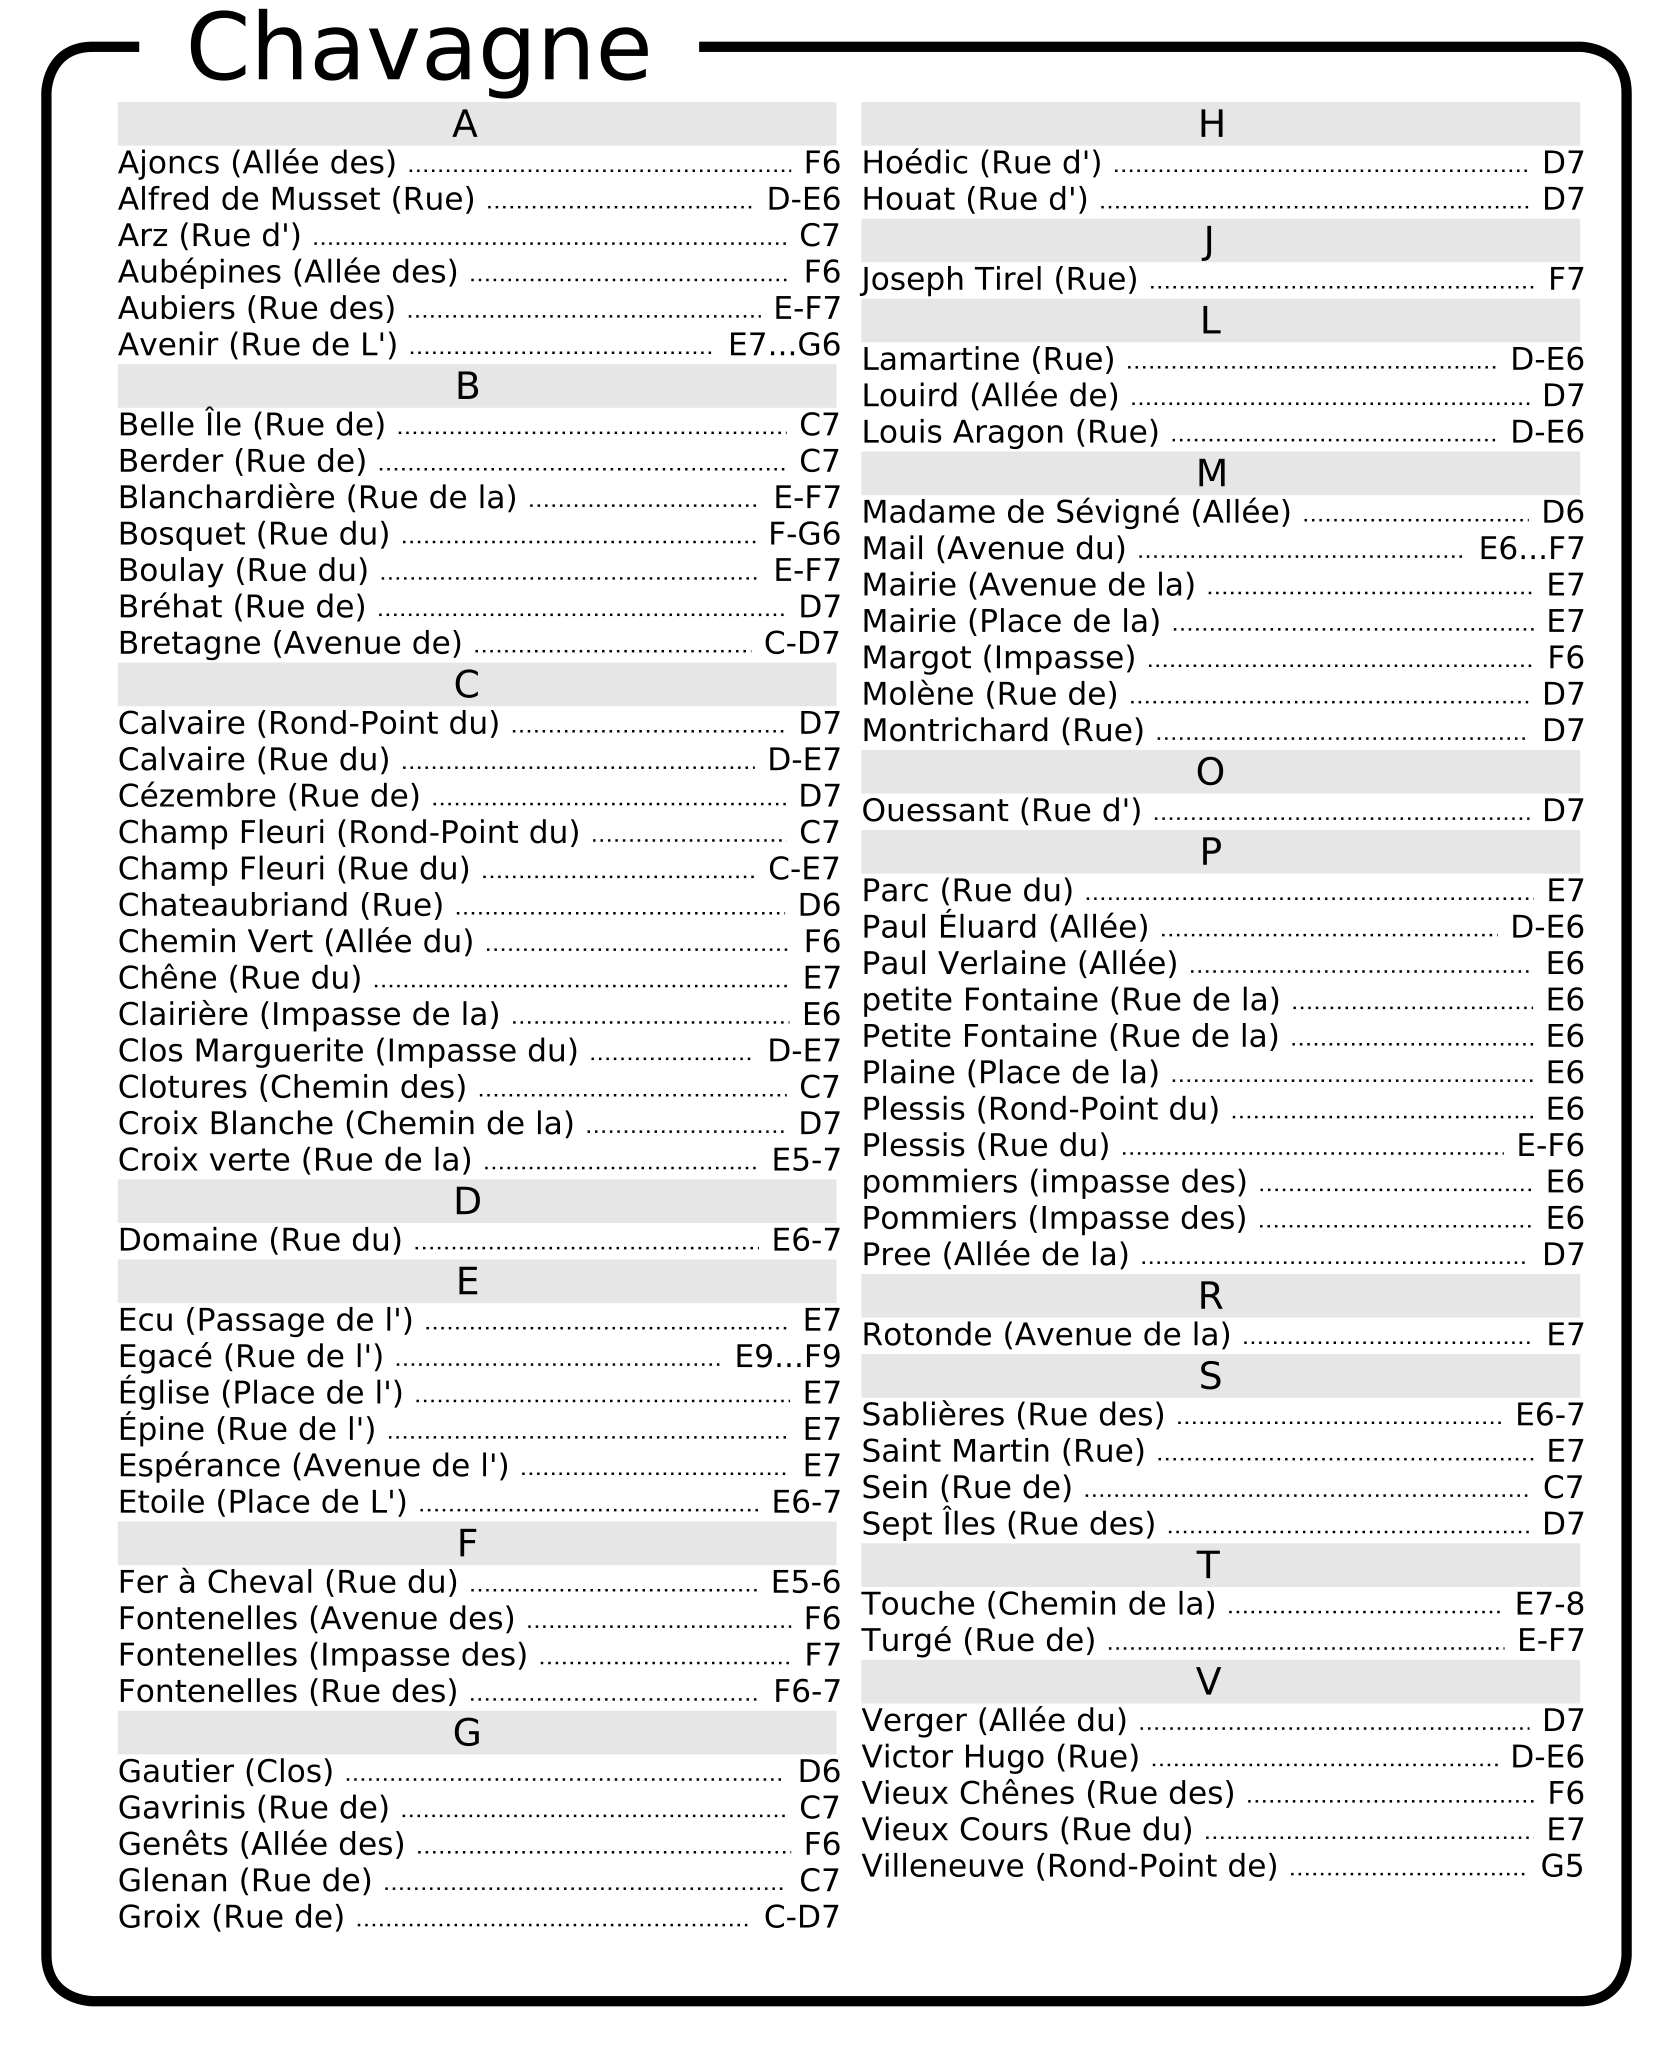
\includegraphics[height=0.8\textheight]{chavagne_index.png}
  \end{center}
\end{frame}

\begin{frame}{Hackfest \#0 details}
  \begin{center}
    \includegraphics[height=0.5\textheight]{chavagne_detail.png}
    \includegraphics[height=0.5\textheight]{chavagne_index_detail.png}
  \end{center}
\end{frame}

\begin{frame}{Hackfest \#1}
  \begin{itemize}
  \item December 2009, near Paris, France
  \item Five developers, four days
  \item Features implemented
    \begin{itemize}
    \item Coverage of the whole world: required a much larger import
      of OSM data
    \item OSM database updated on a daily basis
    \item i18 infrastructure to adapt the street index generation on a
      per-language basis
    \item City name search based on Nominatim
    \item Amenities (schools, town hall, post offices) in the index
    \end{itemize}
  \item All improvements put in production early January 2010
  \item After this hackfest, we started receiving a lot of
    contributions to translate the language and the street index
    rendering logic.
  \end{itemize}
\end{frame}

\begin{frame}{Hackfest \#2}
  \begin{columns}
    \column{0.7\textwidth}
  \begin{itemize}
  \item August 2010, Toulouse, France
  \item Six developers, seven days
  \item Features
    \begin{itemize}
    \item Complete rewrite of the rendering engine, to support
      multiple layouts (index on the same side as the map, at the
      bottom or on the side) and selectable standard paper sizes
    \item Support for multiple stylesheets (style of renderings)
    \item Major rewrite of the web interface, to provide a wizard for
      the map creation
    \end{itemize}
  \item Features not completed, so no delivery in production...
  \end{itemize}
  \column{0.3\textwidth}
  \includegraphics[height=0.5\textheight]{hackfest-2-notes.jpg}
  \end{columns}
\end{frame}

\begin{frame}{Hackfest \#2 result}
  \begin{center}
    \includegraphics[height=0.8\textheight]{stains.png}
  \end{center}
\end{frame}

\begin{frame}{Hackfest \#2 result}
  \begin{center}
    \includegraphics[height=0.8\textheight]{arabic-index.png}
  \end{center}
\end{frame}

\begin{frame}{Server migration, october 2010}
  Our initial server, having 250 GB of hard disk space, was completely
  filled with the OpenStreetMap database.\\

  Had to migrate all our services on different machines, causing a
  severe downtime for the service.
\end{frame}

\begin{frame}{Hackfest \#3}
  \begin{columns}
    \column{0.6\textwidth}
  \begin{itemize}
  \item February 2012, San Francisco, USA
  \item Four developers, two days
  \item Things done
    \begin{itemize}
    \item Investigation of a Mapnik rendering bug that was a block for
      releasing in production our new version
    \item Add some monitoring tools on our servers
    \item Polish web interface details
    \end{itemize}
  \item Improvements made in August 2010 were still not in production!
  \end{itemize}
    \column{0.4\textwidth}
  \includegraphics[width=0.9\textwidth]{hackfest-3.jpg}
  \end{columns}
\end{frame}

\begin{frame}{Hackfest \#4}
  \begin{columns}
    \column{0.6\textwidth}
  \begin{itemize}
  \item March 2012, Rennes, France
  \item Five developers, seven days
  \item Objective: put in production all the new features
    \begin{itemize}
    \item Support for multi-page maps, which allows to render large
      maps on A4 and A5 paper sizes
    \item Integration of several Mapnik stylesheets
    \item Many, many fixes in the rendering engine and the web
      interface
    \end{itemize}
  \item {\bf On April, 19th, a few weeks after the hackfest, we
      managed to put all the improvements in production and make it
      public!}
  \end{itemize}
    \column{0.4\textwidth}
  \includegraphics[width=0.9\textwidth]{hackfest-4.jpg}
  \end{columns}
\end{frame}

\begin{frame}{Hackfest \#4 results}
  \begin{center}
    \includegraphics[height=0.8\textheight]{chavagne-multi-page-front.png}
    \includegraphics[height=0.8\textheight]{chavagne-multi-page-overview.png}
  \end{center}
\end{frame}

\begin{frame}{Using maposmatic.org (1/11)}
  \begin{center}
    \includegraphics[width=\textwidth]{screenshot1.png}
  \end{center}
\end{frame}

\begin{frame}{Using maposmatic.org (2/11)}
  \begin{center}
    \includegraphics[width=\textwidth]{screenshot2.png}
  \end{center}
\end{frame}

\begin{frame}{Using maposmatic.org (3/11)}
  \begin{center}
    \includegraphics[width=\textwidth]{screenshot3.png}
  \end{center}
\end{frame}

\begin{frame}{Using maposmatic.org (4/11)}
  \begin{center}
    \includegraphics[width=\textwidth]{screenshot4.png}
  \end{center}
\end{frame}

\begin{frame}{Using maposmatic.org (5/11)}
  \begin{center}
    \includegraphics[width=\textwidth]{screenshot5.png}
  \end{center}
\end{frame}

\begin{frame}{Using maposmatic.org (6/11)}
  \begin{center}
    \includegraphics[width=\textwidth]{screenshot6.png}
  \end{center}
\end{frame}

\begin{frame}{Using maposmatic.org (7/11)}
  \begin{center}
    \includegraphics[width=\textwidth]{screenshot7.png}
  \end{center}
\end{frame}

\begin{frame}{Using maposmatic.org (8/11)}
  \begin{center}
    \includegraphics[width=\textwidth]{screenshot8.png}
  \end{center}
\end{frame}

\begin{frame}{Using maposmatic.org (9/11)}
  \begin{center}
    \includegraphics[width=\textwidth]{screenshot9.png}
  \end{center}
\end{frame}

\begin{frame}{Using maposmatic.org (10/11)}
  \begin{center}
    \includegraphics[width=\textwidth]{screenshot10.png}
  \end{center}
\end{frame}

\begin{frame}{Using maposmatic.org (11/11)}
  \begin{center}
    \includegraphics[width=\textwidth]{screenshot11.png}
  \end{center}
\end{frame}

\begin{frame}{OSM Database (1/2)}
  \begin{itemize}
  \item In order to render maps, Mapnik needs an OSM database
    converted in a PostGIS schema
  \item The format of the main OSM database is different, to allow
    flexible tags: the conversion process is non-trivial
  \item {\bf Initial import}
    \begin{itemize}
    \item Planet dumps available in a protobuf-encoded format, at
      \url{http://planet.openstreetmap.org/pbf/}
    \item Converted to the PostGIS schema and pushed into a PostgreSQL
      database by the {\em osm2pgsql} tool,
      \url{http://wiki.openstreetmap.org/wiki/Osm2pgsql}
    \item Takes 8-10 days on a 6x4 cores Xeon X5670 @ 2.93 Ghz, 24 GB
      of RAM, a single hard drive
    \item Initial file 16 GB, resulting database around 250 GB
    \end{itemize}
  \end{itemize}
\end{frame}

\begin{frame}{OSM Database (2/2)}
  \begin{itemize}
  \item {\bf Regular updates}
    \begin{itemize}
    \item Minutely updates available. At MapOSMatic, we group them by
      slots of 15 minutes.
    \item Generated using the {\em osmosis} tool, from the
      \url{http://planet.openstreetmap.org/redaction-period/minute-replicate/}
      server
    \item \url{http://wiki.openstreetmap.org/wiki/Osmosis}
    \item Applied to the PostgreSQL database using {\em osm2pgsql}
    \item Very hard to keep updated: time to apply a 15 minutes update
      is often around 10 minutes
    \end{itemize}
  \item Need to buy a SSD drive.
  \end{itemize}
\end{frame}

\begin{frame}{OSM Database diagram}
  \begin{center}
    \includegraphics[width=\textwidth]{osm-database.pdf}
  \end{center}
\end{frame}

\begin{frame}{OCitySMap}
  \begin{itemize}
  \item OCitySMap is a Python module that implements the map and
    street index rendering
  \item A command-line client is provided
  \item Uses multiple Python modules:
    \begin{itemize}
    \item {\bf psycopg2} for direct PostgreSQL queries used to build
      the index of streets and amenities
    \item {\bf mapnik} to do the map rendering
    \item {\bf pango} to do the text rendering
    \item {\bf cairo} to layout the map and index
    \item {\bf ogr} for shapes manipulation
    \end{itemize}
  \item Available as a separate project from MapOSMatic
  \end{itemize}
\end{frame}

\begin{frame}{OCitySMap architecture}
  \begin{center}
    \includegraphics[height=0.8\textheight]{ocitysmap.pdf}
  \end{center}
\end{frame}

\begin{frame}[fragile]{OCitySMap example usage}
Render an administrative boundary, knowing its OSM id:
\begin{verbatim}
./render.py -t "Chevreuse" -f pdf -s mapquest_eu \
            -L fr_FR -l multi_page --paper-format A4 \
            --osmid=-943886
\end{verbatim}
Render a geographic area, knowing its bounding box:
\begin{verbatim}
  ./render.py -t "Map Title" \
              -b 48.7268,1.9946 48.6801,2.0742
\end{verbatim}
\end{frame}

\begin{frame}{OCitySMap installation in a nutshell}
  \begin{enumerate}
  \item Install PostgreSQL and PostGIS, create a PostgreSQL user and
    database
  \item Enable PostGIS in the database
  \item Build and install {\em osm2pgsql}
  \item Download and import the OSM data with {\em osm2pgsql}
  \item Install Mapnik
  \item Install Mapnik-OSM, the official OpenStreetMap stylesheet for
    Mapnik. Requires downloading of coast line data and fonts.
  \item Installation and configuration of OCitySMap
  \end{enumerate}
  Fortunately, everything is documented in details in the
  \path{INSTALL} file of the project.
\end{frame}

\begin{frame}{MapOSMatic}
  MapOSMatic is composed of:
  \begin{enumerate}
  \item {\bf A Web interface}, written using the Django
    framework. This
    interface allows user to create new maps, view existing maps, etc.\\
    When a new map is requested, it is put into a rendering queue.
  \item {\bf A daemon}, which processes the jobs in the rendering
    queue one by one. This daemon uses {\em OCitySMap} to do the
    rendering.
  \end{enumerate}
  \begin{center}
    \includegraphics[width=\textwidth]{maposmatic.pdf}
  \end{center}
\end{frame}

\begin{frame}{Languages}

  Both the website and the street index logic requires
  translations. So far, we have translations in:
  \begin{columns}
    \column{0.5\textwidth}
    \begin{itemize}
    \item French
    \item Dutch
    \item German
    \item Spanish
    \item Brazilian Portuguese
    \item Russian
    \end{itemize}
    \column{0.5\textwidth}
    \begin{itemize}
    \item Norvegian Bokmal
    \item Italian
    \item Catalan
    \item Hungarian
    \item Polish
    \item Indonesian
    \item Arabic
    \end{itemize}
  \end{columns}
\end{frame}

\begin{frame}{Hardware setup}
  \begin{center}
    \includegraphics[width=\textwidth]{hardware-setup.pdf}
  \end{center}
\end{frame}

\begin{frame}{Statistics}
  \begin{itemize}
    \item {\bf 50000 maps} render since the service has been launched
    \item {\bf 5000 to 10000} visitors per month
    \item {\bf 280 GB} of OSM database
  \end{itemize}
  \begin{center}
    \includegraphics[width=0.8\textwidth]{maposmatic-stats.png}\\
    Number of daily maps rendered
  \end{center}
\end{frame}

\begin{frame}{Example of usage}
  \begin{center}
    \includegraphics[width=0.7\textwidth]{orange-city.jpg}\\
    City of {\em Orange, France}, has printed folded maps using
    MapOSMatic.
  \end{center}
\end{frame}

\begin{frame}{Future work}
  \begin{itemize}
  \item Allow users to customize the set of amenities and point of
    interests visible in the index
  \item Allow users to customize the rendering style. Maybe by
    exploring the {\em MapCSS} technology.
  \item Add a legend and scale on the map.
  \item Add more translations
  \item Fix more bugs
  \end{itemize}
\end{frame}

\begin{frame}{Join the project!}
  \begin{itemize}
  \item {\bf Website}: \url{http://www.maposmatic.org}
  \item {\bf Blog}: \url{http://news.maposmatic.org}
  \item {\bf Savannah project}: \url{https://savannah.nongnu.org/projects/maposmatic/}
  \item {\bf Git} repositories
    \begin{itemize}
      \scriptsize
    \item OcitySMap: \url{git://git.savannah.nongnu.org/maposmatic/ocitysmap.git}
    \item MapOSMatic: \url{git://git.savannah.nongnu.org/maposmatic.git}
    \end{itemize}
  \item {\bf Mailing list}: \url{https://lists.nongnu.org/mailman/listinfo/maposmatic-dev}
  \item {\bf IRC channel}: {\tt \#maposmatic} on {\em Freenode}
  \end{itemize}
\end{frame}

\begin{frame}{Conclusion}
  \begin{itemize}
  \item The OSM database and all the tools around it allow a
    relatively {\bf easy access to geographic data}
  \item {\bf Very impressive amount of reuse} in this project, thanks to the
    numerous Python modules available.
  \item MapOSMatic is, we think, a {\bf good illustration of what is
    possible thanks to freely available data}
  \item MapOSMatic is free software, {\bf join us and contribute}!
  \end{itemize}
\end{frame}

\begin{frame}
  \begin{center}
    \Huge
    Questions ?\\
    \Large
    \vspace{2cm}
    \path{http://www.maposmatic.org}\\
    \vspace{2cm}
    \normalsize
    \path{thomas.petazzoni@enix.org}\\
    \path{contact@maposmatic.org}\\
  \end{center}
\end{frame}

\end{document}
